\documentclass[11pt]{article}
\usepackage[margin=1in]{geometry}
\usepackage{../../styles/isaiah}
\usepackage{../../styles/components/configurableGrid}
% Hebrew font configuration is now provided by the main style package

\begin{document}

\newpage
\begin{center}
{\Huge\bfseries Isaiah 1:2-31}
\end{center}
\vspace{10pt}
% Overview of Isaiah 1-12 Chiastic Structure
\isaiahChiasticOverview{1}
% Overview of Isaiah 1
\begin{overview}{Isaiah 1:2-31 — Overview}

\overviewsection[0]{%
\textbf{Verses 2-9: Rebellious Children}
\begin{itemize}
    \item Israel has rebelled against God despite His care for them
    \item Their land is consumed like \highlightred{Sodom and Gomorrah}
    \item A \boldred{sinful} people who have \highlightbrown{forsaken the LORD}
\end{itemize}
}

\overviewsection[1]{%
\textbf{Verses 10-17: Empty Religion}
\begin{itemize}
    \item God rejects their sacrifices and festivals that lack true \highlightblue{justice} and \highlightaqua{righteousness}
\end{itemize}
}

\overviewsection[2]{%
\textbf{Verses 18-20: A Choice}
\begin{itemize}
    \item Obedience leads to blessing
    \item Rebellion leads to judgment
\end{itemize}
}

\overviewsection[1]{%
\textbf{Verses 21-26: City of Faithfulness}
\begin{itemize}
    \item True \highlightblue{justice} and \highlightaqua{righteousness} makes the city faithful
\end{itemize}
}

\overviewsection[0]{%
\textbf{Verses 27-31: Fire of Justice}
\begin{itemize}
    \item A \boldred{sinful} people who have \highlightbrown{forsaken the LORD}
    \item Those who repent will be redeemed through \highlightblue{justice} and \highlightaqua{righteousness} but those who don't...
    \item ...their land is consumed like \highlightred{Sodom and Gomorrah}
\end{itemize}
}

\end{overview}

% Verses 2-9
\begin{biblicaloutline}[Isaiah 1:2-9]
    
    \subsectionheader{Rebellious Children (2-4)}

    \begin{versesection}{2em}
        \versenum{2} \highlightgreen{Hear}, O heavens, and \textcolor{highlightgreen}{give ear}, O earth;
        \poetryline for the LORD has spoken:
 ``Children have I reared and brought up,
\poetryline but they have rebelled against me.

\versenum{3}  The ox knows its owner,
\poetryline and the donkey its master's crib,
but Israel does not know,
\poetryline my people do not understand.''

\versenum{4} Ah, \boldred{sinful} nation,
\poetryline a people laden with iniquity,
offspring of evildoers,
\poetryline children who deal corruptly!
They have \highlightbrown{forsaken the LORD},
\poetryline they have despised the Holy One of Israel,
\poetryline they are utterly estranged.
    \end{versesection}
    
    \subsectionheader{Totally Wounded (5-6)}
    
    \begin{versesection}{2em}
        \versenum{5} (a) Why will you still be \textbf{struck down}?
        \poetryline (a') Why will you continue \textbf{to rebel}?
        The whole head is sick,
        \poetryline and the whole heart faint.
        
        \versenum{6} From the sole of the foot even to the head,
        \poetryline there is no soundness in it,
        but bruises and sores
        \poetryline and raw wounds;
        they are not pressed out or bound up
        \poetryline or softened with oil.
    \end{versesection}
    
    \subsectionheader{Desolate Land (7-9)}
    
    \begin{versesection}{2em}
        \versenum{7} Your country lies desolate;
        \poetryline your cities are burned with fire;
        in your very presence
        \poetryline foreigners devour your land;
        \poetryline it is desolate, as \textcolor{highlightred}{overthrown} by foreigners.
        
        \versenum{8} And the daughter of Zion is left
        \poetryline like a booth in a vineyard,
        like a lodge in a cucumber field,
        \poetryline like a besieged city.

        \versenum{9} If the LORD of hosts
        \poetryline had not left us a few survivors,
        we should have been like \highlightred{Sodom},
        \poetryline and become like \highlightred{Gomorrah}.
    \end{versesection}

\end{biblicaloutline}

{\large\bfseries Cosmic Introduction}
{\vspace{1em}}

The summoning of the heavens and the earth to witness the LORD's case is a callback to the Song of Moses in Deuteronomy 32.
It was here where Israel was about to enter the promised land and Moses communicates all of the potential blessings and curses
if they obey or disobey the LORD.

Isaiah is calling out that what is happening/about to happen to Israel is the fulfillment of his prophecy.
{\vspace{1em}}

    \subsectionheader{Deuteronomy 32:1}

    \begin{versesection}{2em}

\versenum{1} "\textcolor{highlightgreen}{Give ear}, O heavens, and I will speak,
\poetryline and let the earth \highlightgreen{hear} the words of my mouth.
\end{versesection}
{\vspace{1em}}
This isn't the only comparison between Deuteronomy 32 and Isaiah 1 either, Isaiah pulls a ton from that passage to prove this point further.

\begin{comparisontable}{Deuteronomy 32}{Isaiah 1}{Notes}

\verserow{
\versenum{1} ``\highlightgreen{Give ear}, O heavens, and I will speak,\\
\hspace*{2em} and let the earth \highlightgreen{hear} the words of my mouth.
}{
\versenum{2a} \highlightgreen{Hear}, O heavens, and \highlightgreen{give ear}, O earth;\\
\hspace*{2em} for the LORD has spoken:
}{
Cosmic Witnesses}

\verserow{
\versenum{5} They have dealt corruptly with him;\\
\hspace*{2em} they are no longer \highlightyellow{his children} because they are blemished;\\
\hspace*{2em} they are a crooked and twisted generation.
}{
\versenum{2b-4} ``\highlightyellow{Children} have I reared and brought up,\\
\hspace*{2em} but they have rebelled against me... they are utterly estranged.''
}{
Estranged Children
}

\verserow{
\versenum{22} For a \highlightorange{fire} is kindled by my anger,\\
\hspace*{2em}	and it burns to the depths of Sheol,\\
devours the earth and its increase,\\
\hspace*{2em}	and sets on fire the foundations of the mountains.
}
{
\versenum{31} And the strong shall become tinder,\\
\hspace*{2em} and his work a spark,\\
 and both of them shall \highlightorange{burn} together,\\
\hspace*{2em} with none to quench them.
}{
Consuming Fire
}

\verserow{
\versenum{32} For their vine comes from the vine of \highlightred{Sodom}\\
\hspace*{2em} and from the fields of \highlightred{Gomorrah};
}{
\versenum{9-10} ``we should have been like \highlightred{Sodom}...\\
\hspace*{2em} you rulers of \highlightred{Sodom}! you people of \highlightred{Gomorrah}!''
}{
Sodom and Gomorrah
}
\verserow{
\versenum{41} Behold, I will repay. \highlightpurple{Vengeance} is mine, and recompense,\\
}{
       \versenum{24b} ``Ah, I will get relief from my enemies\\
       \hspace*{2em} and \highlightpurple{avenge} myself on my foes.
 }{
       Vengeance on enemies
}
\end{comparisontable}
{\vspace{2em}}
{\large\bfseries Sodom and Gomorrah}
{\vspace{1em}}

The whole of verses 7-9 set up for the punchline of verse 10. We can get hints that Isaiah is making
the comparison to Sodom and Gomorrah through "burned with fire" and "overthrown". "Overthrown" is only ever
used elsewhere in the Bible with reference to God overthrowing Sodom and Gomorrah.

{\vspace{1em}}
If this is the case, what is that saying about Israel? What is that saying about the about the "foreigners"?


% Verses 10-15
\begin{biblicaloutline}[Isaiah 1:10-17]

    \begin{versesection}{2em}
\versenum{10} \highlightgreen{Hear} the word of the LORD, you rulers of \highlightred{Sodom}!
\poetryline \textcolor{highlightgreen}{Give ear} to the teaching of our God, you people of \highlightred{Gomorrah}!

\versenum{11} ``What to me is the multitude of your sacrifices? says the LORD;
\poetryline I have had enough of burnt offerings of rams
\poetryline and the fat of well-fed beasts;
I do not delight in the blood of bulls,
\poetryline or of lambs, or of goats.

\versenum{12} When you come to appear before me,
\poetryline who has required of you this trampling of my courts?

\versenum{13} Bring no more vain offerings;
\poetryline incense is an abomination to me.
New moon and Sabbath and the calling of convocations---
\poetryline I cannot endure iniquity and solemn assembly.

\versenum{14} Your new moons and your appointed feasts my soul hates;
\poetryline they have become a burden to me;
\poetryline I am weary of bearing them.

\versenum{15} When you spread out your hands,
\poetryline I will hide my eyes from you;
even though you make many prayers,
\poetryline I will not \highlightgreen{listen};
\poetryline your hands are full of blood.

\versenum{16} Wash yourselves; make yourselves clean;
\poetryline remove the evil of your deeds from before my eyes;
\poetryline cease to do evil,

\versenum{17} learn to do good; seek \highlightblue{justice}, correct oppression;
\poetryline bring \highlightblue{justice} \boldblue{to the fatherless},
\poetryline \boldblue{plead the widow's cause}.
    \end{versesection}

\end{biblicaloutline}
{\vspace{4em}}
{\large\bfseries Bad Sacrifices}
{\vspace{1em}}

The LORD is saying that he's burdened by their sacrifices and who even asked them to do so, when there's a decent
bit of Scripture pointing to \textit{Him} being the one who commaned it in the first place!

{\vspace{1em}}
There's something more needed than just their sacrifices and it all culminates in verses 16-17. None of their sacrifices or festivals
mean anything to the LORD if they are devoid of social justice.

{\vspace{3em}}

{\large\bfseries Bloody Hands}
{\vspace{1em}}

Pretty cool poetry on line 15. The "hands full of blood" refers to prayerful hands that either could have:
\begin{itemize}
    \item been covered in blood from all of the sacrifices they were making
    \item been covered in blood from murder (Gen. 4:10-11)
\end{itemize}
{\vspace{1em}}

\hebrewword{Justice}{מִשְׁפָּט}{mish.pat}{God's right order in the world.}

People treated as equal before his eyes. The oppressed and poor are lifted up. The proud and murderers brought low.

So how are God's children supposed to clean themselves? Removing evil, doing good, seeking justice for orphans and widows

% Verses 18-20
\begin{biblicaloutline}[Isaiah 1:18-20]

    \begin{versesection}{2em}
\versenum{18} ``Come now, let us reason together, says the LORD:
\poetryline though your \boldred{sins} are like scarlet,
\poetryline they shall be as white as snow;
though they are red like crimson,
\poetryline they shall become like wool.

\versenum{19} If you are willing and \highlightgreen{obedient},
\poetryline you shall eat the good of the land;

\versenum{20} but if you refuse and rebel,
\poetryline you shall be eaten by the sword;
\poetryline for the mouth of the LORD has spoken.''
    \end{versesection}

\end{biblicaloutline}


{\vspace{4em}}
{\large\bfseries Just Obey?}
{\vspace{1em}}

How is Israel going to have their sins cleaned? Their hands are bloody and full of murder! It seems like v19-20 is repeating the message of "Obey Yahweh" as the solution?
\\\\
Israels been given this instruction already before though! They've been told to show justice and righteousness, so will this one more command be exactly what they need? Or will they need someone to do this on their behalf? Reading further in Isaiah will show us through Whom this will be done for them.


\newpage
% Verses 21-26 - Using chiastic structure
\begin{chiasticoutline}[Isaiah 1:21-26]{.75em}{2em}

    \chiasticverse[A]{0}{
\versenum{21} How the faithful city has become a whore,

\poetryline she who was full of \highlightblue{justice}!

\highlightaqua{Righteousness} lodged in her,

\poetryline but now murderers.
    }

    \chiasticverse[B]{1}{
\versenum{22} Your silver has become \highlightsilver{dross},

\poetryline your best wine mixed with water.
    }

    \chiasticverse[C]{2}{
\versenum{23} Your princes are rebels and companions of thieves.

\poetryline Everyone loves a bribe and runs after gifts.

(a) They do not bring \highlightblue{justice} \boldblue{to the fatherless},

(a')\poetryline and \boldblue{the widow's cause} does not come to them.
    }

    \chiasticverse[C']{2}{
\versenum{24} Therefore the Lord declares,

\poetryline the LORD of hosts, the Mighty One of Israel:

``Ah, I will get relief from my enemies

\poetryline and avenge myself on my foes.
    }

    \chiasticverse[B']{1}{
\versenum{25} I will turn my hand against you

\poetryline and will smelt away your \highlightsilver{dross} as with lye

\poetryline and remove all your alloy.
    }

    \chiasticverse[A']{0}{

\versenum{26} And I will restore your \highlightblue{judges} as at the first,

\poetryline and your counselors as at the beginning.

Afterward you shall be called the city of \highlightaqua{righteousness},

\poetryline the faithful city.''
    }

\end{chiasticoutline}
\hebrewword{Righteousness}{צְדָקָה}{tse.da.qah}{Right relationships with God and others}
\begin{quote}
\textit{"The meaning of tsedeqah is an ethical standard of right relationship. Biblical scholar J. Alec
Motyer defines its use as "right with God and therefore committed to putting right all other relationships in life," and "to do right by someone."
\\\\Tsedeqah is the standard of right relationship between all people. And mishpat is the action you
take to create the standard of tsedeqah. Biblical righteousness is about right relationships in
day-to-day conduct in family, work, and community"}\\\\
\hfill --- Bible Project, \textit{Justice Study Notes}, https://bibleproject.com/videos/justice/
\end{quote}

% Verses 27-31 - Using chiastic structure
\begin{chiasticoutline}[Isaiah 1:27-31]{.25em}{2em}

    \chiasticverse[A]{0}{
\versenum{27} Zion shall be redeemed with \highlightblue{justice},

\poetryline and her converts with \highlightaqua{righteousness}.

\versenum{28} But rebels and \boldred{sinners} shall be broken together,

\poetryline and those who \highlightbrown{forsake the LORD} shall be consumed.

    }

    \chiasticverse[B]{1}{
        \versenum{29} For they shall be ashamed of the oaks that you desired;

\poetryline and you shall blush for the gardens that you have chosen.
    }

    \chiasticverse[B']{1}{
\versenum{30} For you shall be like an oak whose leaf withers,

\poetryline and like a garden without water.
    }

    \chiasticverse[A']{0}{
\versenum{31} And the strong shall become tinder,

\poetryline and his work a spark,

and both of them shall burn together,

\poetryline with none to quench them.
    }

\end{chiasticoutline}
{\vspace{2em}}
{\large\bfseries Desirable Trees}
{\vspace{1em}}

Only one other time in the whole Hebrew Bible does the word for "desire" (\hebrew{חָמַד} – kha.mad) appear in reference to desiring trees.
It is in Genesis 3:6 when Eve saw that the tree of the knowledge of good and evil was desirable to make one wise.

{\vspace{1em}}
Just like the root of all sin is a desire to ignore God's Words (not "shema" to Yahweh) and take our own wisdom for ourselves,
so is Israel's sin here. As highlighted in prior sections, they're giving vain sacrifices that might seem good in their eyes,
but they're missing the whole point – true worship requires justice and righteousness – right relationships between both God and others.

{\vspace{2em}}
{\large\bfseries Conclusion}
{\vspace{1em}}

So if this is the state of Israel, what hope do they have? How can this Israel be redeemed as Isaiah says will happen in v27?
\\\\
In Chapter 2, we get a picture of what the result of this redemption and judgement will look like.

\begin{thesauce}
\sauceitem{In v6, there is no "soundness" in Zion. The Hebrew word \hebrew{מְתֹם} me.tom has the same root for "unblemished" or "whole". This is the same word used of the spotless lamb sacrifice needed for their coverings. How could we compare the "blemished" natrue of Israel in light of their "blemished" sacrifices?}

\sauceitem{In v13, just about every other time the word "convocations" is used in the Hebrew Bible, it has the word "holy" before it. Not these convocations! Could look into other usages in the Scriptures or even read more of the Levitical laws showing how they're supposed to be done.}
    
\sauceitem{There's a lot of "courtroom" language in this passage. It's almost as if Yahweh is pleading His case. He picks this theme back up in chapter 5 as well – "What more could I have done?"}

\sauceitem{We'll probably end up touching on this later in Isaiah, but the concept of a "city" is usually not thought of in the way we do today. The very first city mentioned in the Bible was built by Cain after his sin and exiling.}

\end{thesauce}
\newpage{}
\begin{center}
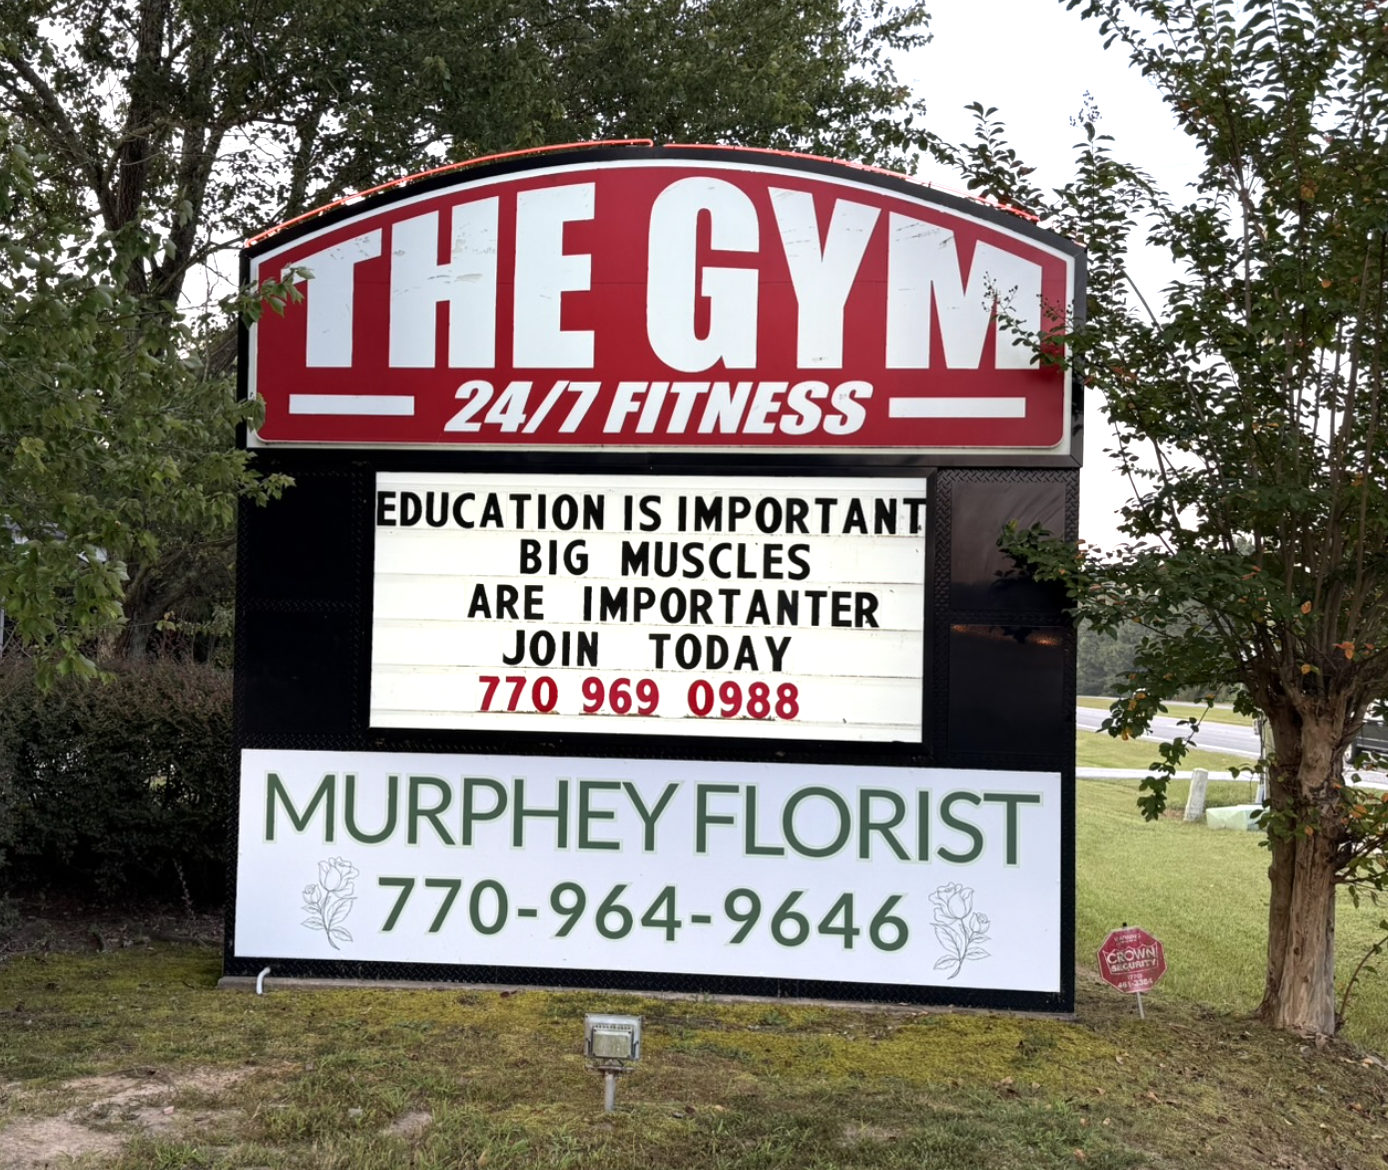
\includegraphics[width=1\textwidth]{parallelism.png}
\end{center}
\vspace{5em}
{\Huge a) \textcolor{cyan}{Education} is \textcolor{brown}{Important}}
\\\\\\
{\Huge a') \textcolor{cyan}{Big Muscles} are \textcolor{brown}{Importanter}}

\begin{center}
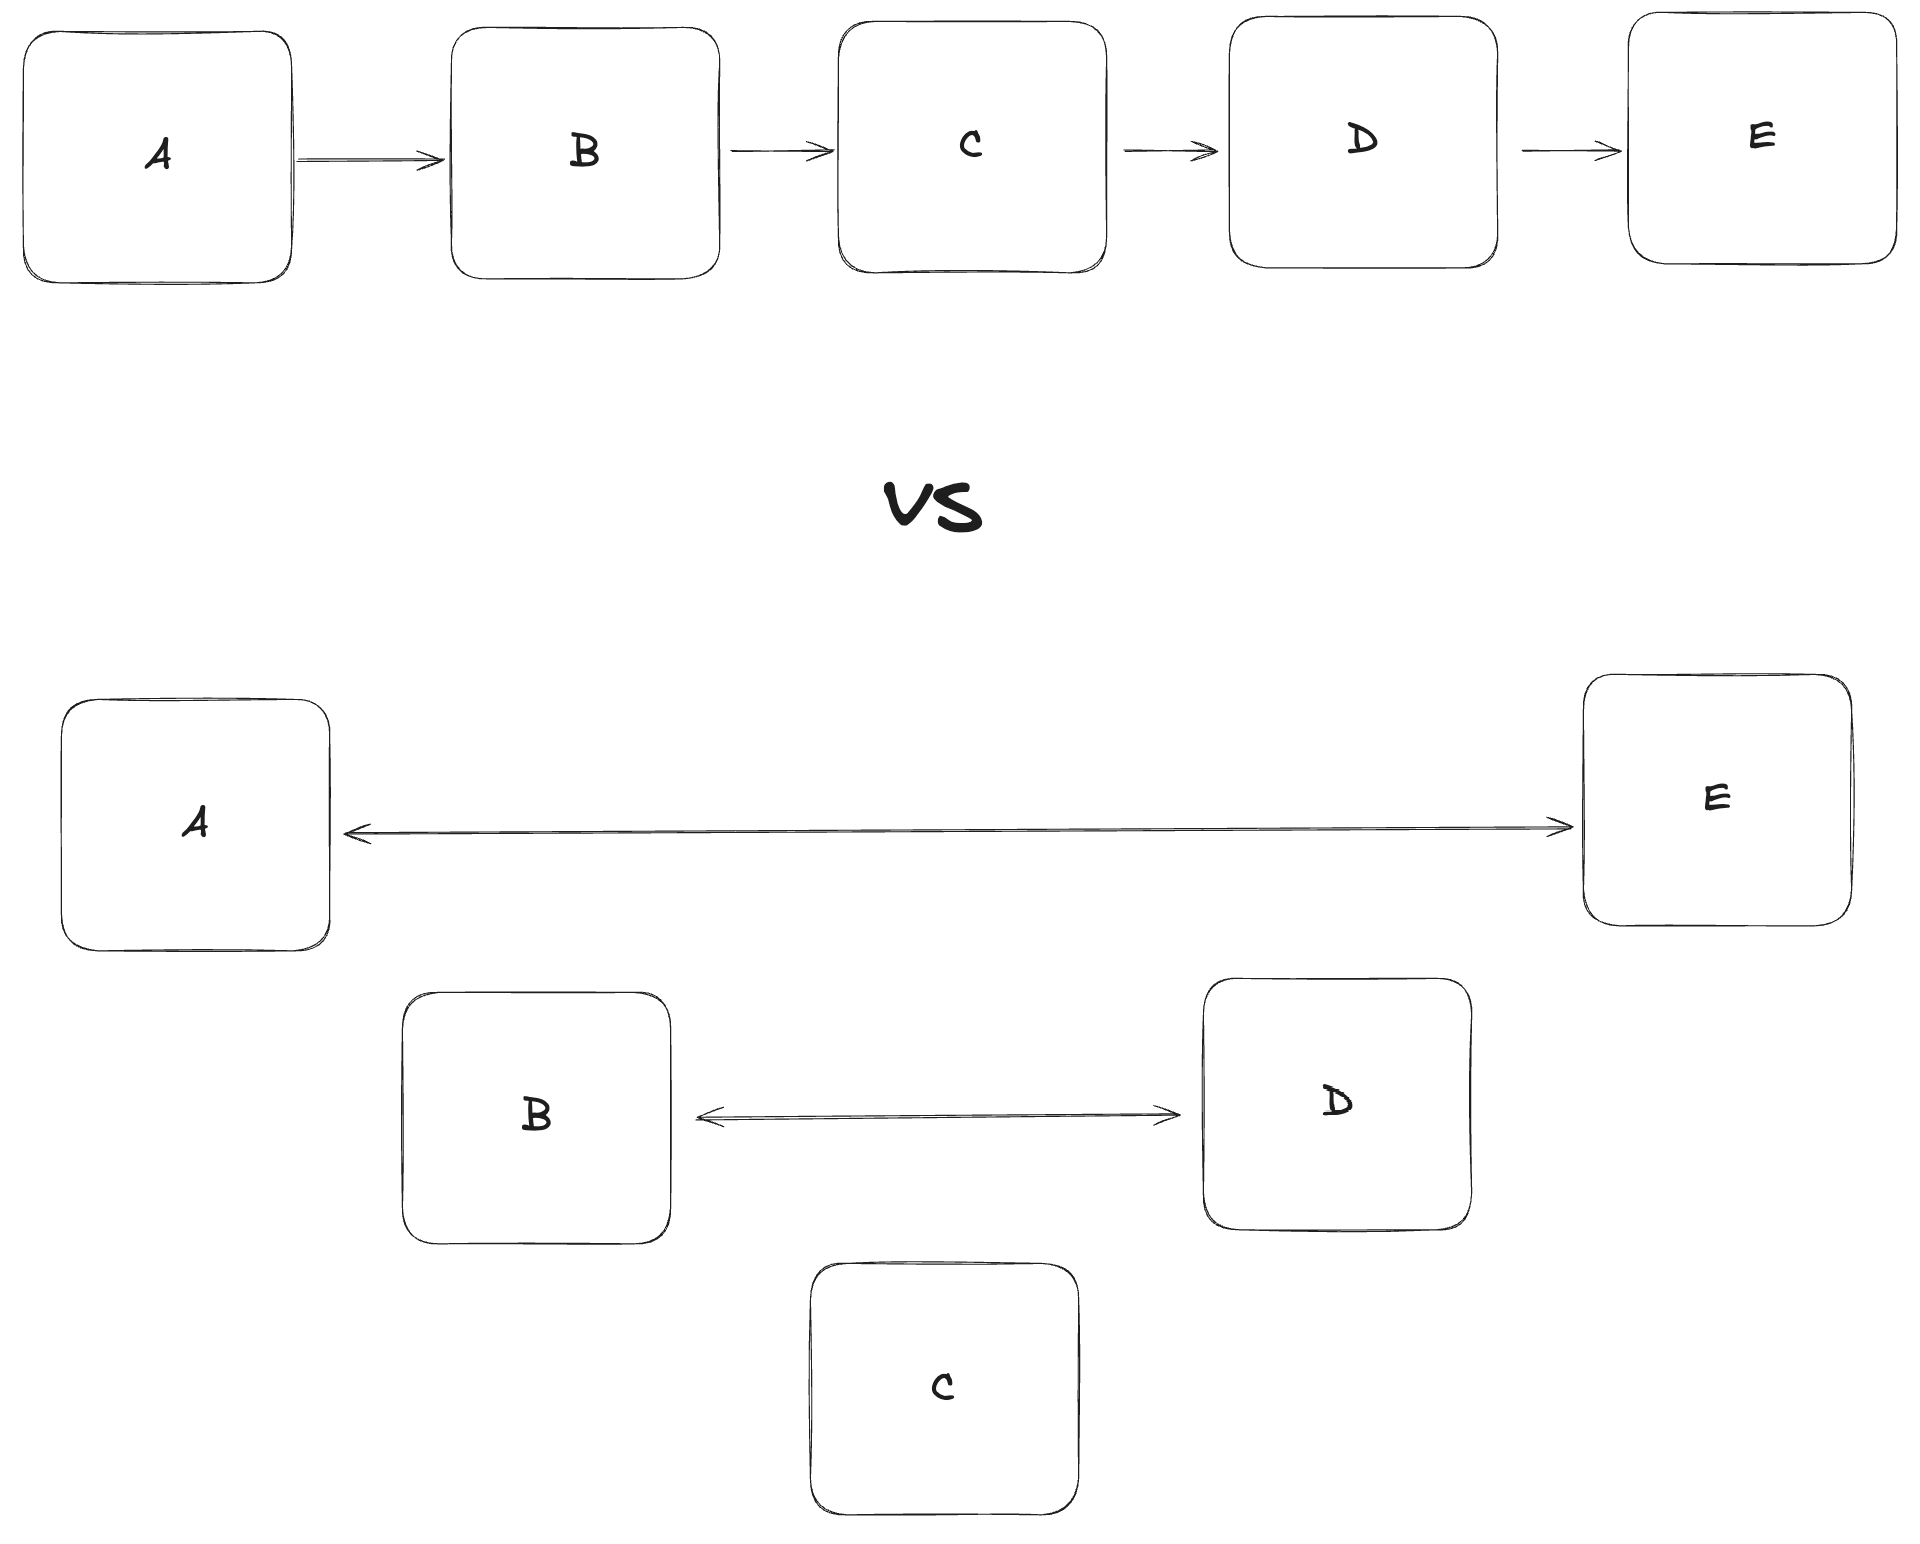
\includegraphics[width=1\textwidth]{reading-difference.png}
\end{center}
\end{document}